\section{ZLP parametrisation for vacuum spectra}
\label{sec:results_vacuum}

Now we move to present the application of the strategy presented in the previous
section to the parametrisation of ZLP spectra acquired in vacuum.
%
Applying our model to this case has a two-fold motivation.
%
First of all, we aim to demonstrate that our model is flexible enough to effectively reproduce the
input EELS measurements for a range of variations of the operation parameters of the microscope.
%
Second, it will allow us to provide a calibration prediction
useful for the case of the in-sample measurements.
%
Such calibration is necessary since, as explained in Sect.~\ref{sec:training}, some of the model
hyper-parameters are determined by the comparison of the intensity derivatives
between spectra taken in vacuum and those in sample.

In this section, first of all we present the input dataset and motivate the choice
of training settings and model hyperparameters.
%
Then we validate the model training by assessing the fit quality.
%
Lastly, we study the dependence of the model predictions in its various input
variables, and study the dependence of the model uncertainties upon
the removal of a subset of the training dataset.

\subsection{Training settings}

In Table~\ref{table:vacuumdata} we collect the main properties of the EELS spectra acquired in vacuum to train the neural
    network model.  For each set of spectra, we indicate the exposure time $t_{\rm exp}$, the beam energy
    $E_b$, the number of spectra $N_{\rm sp}$ recorded for these operation conditions, the number $N_{\rm dat}$ of
    bins in each spectrum, the range in electron energy loss $\Delta E$,
    and the average full width at half maximum (FWHM)
    evaluated over the $N_{\rm sp}$ spectra with the corresponding variance.
    %
    All the spectra  listed on Table~\ref{table:vacuumdata}
    were acquired with a Titan TEM equipped with a Schottky field emitter.
    %
    We point out that since here
    we are interested in the low-loss region, $\Delta E_{\rm max}$ does not need
    to be too large, and in any case the large $\Delta E$ behaviour of the model is fixed
    by the constraint implemented by Eq.~(\ref{eq:chi2modified}).

%%%%%%%%%%%%%%%%%%%%%%%%%%%%%%%%%%%%%%%%%%%%%%%%%%%%%%%%%%%%%%%%%%%%%%%%%%%%%%%%%%%%%%%%%%%%%
%%%%%%%%%%%%%%%%%%%%%%%%%%%%%%%%%%%%%%%%%%%%%%%%%%%%%%%%%%%%%%%%%%%%%%%%%%%%%%%%%%%%%%%%%%%%%
\begin{table}[t]
  \begin{center}
            \renewcommand{\arraystretch}{1.50}
  \begin{tabular}{@{}ccccccccc}
\br
Set & $t_{\rm exp}$ {(}ms{)} & $E_{\rm b}$ {(}keV{)} & $N_{\rm sp}$ & $N_{\rm dat}$ & $\Delta E_{\rm min}$~(eV)  & $\Delta E_{\rm max}$~(eV)  & FWHM~(meV)  \\ 
\mr
1        & 100                 & 200                  & 15          & 2048               & -0.96              & 8.51     & $47\pm7 $         \\
2        & 100                 & 60                   & 7           & 2048               & -0.54              & 5.59    & 
$ 50 \pm 4$         \\
3        & 10                  & 200                  & 6          & 2048               & -0.75              & 5.18      & 
$ 26 \pm 3$         \\
4        & 10                  & 60                   & 6           & 2048               & -0.40              & 4.78       & 
$ 34\pm 2$         \\ 
\br
  \end{tabular}
    \end{center}
  \caption{\small Summary of the main properties of the EELS spectra acquired in vacuum to train the neural
    network model.  For each set of spectra, we indicate the exposure time $t_{\rm exp}$, the beam energy
    $E_b$, the number of spectra $N_{\rm sp}$ recorded for these operation conditions, the number $N_{\rm dat}$ of
    bins in each spectrum, the range in electron energy loss $\Delta E$,
    and the average FWHM evaluated over the $N_{\rm sp}$ spectra with the corresponding standard deviation
  }
   \label{table:vacuumdata}
\end{table}
%%%%%%%%%%%%%%%%%%%%%%%%%%%%%%%%%%%%%%%%%%%%%%%%%%%%%%%%%%%%%%%%%%%%%%%%%%%%%%%%%%%%%%%%%%%%%%%%%5
%%%%%%%%%%%%%%%%%%%%%%%%%%%%%%%%%%%%%%%%%%%%%%%%%%%%%%%%%%%%%%%%%%%%%%%%%%%%%%%%%%%%%%%%%%%%%

    The energy resolution of these spectra, quantified by the value of their FWHM, ranges
    from 26 meV to 50 meV depending on the specific operation conditions of the microscope,
    with an standard deviation between 2 and 7 meV.
    %
    The value of the FWHM varies only mildly with the value of the beam energy $E_b$
    but grows by around a factor two for spectra collected at larger exposure times $t_{\rm exp}$.
    %
    A total of almost $7\times 10^4$ independent measurements will be thus used for the ZLP model
    training on the vacuum spectra.
    %
    As will be highlighted in Sects.~\ref{eq:depdeltae} and~\ref{eq:depebeam}, one of the advantages of our ZLP model is that it can extrapolate its predictions
    to other operation conditions beyond those used for the training.

Following the strategy presented in Sect.~\ref{sec:methodology}, first of all we combine the $N_{\rm sp}$ spectra
corresponding to each of the four sets of operation conditions and determine the statistical uncertainty
associated to each energy loss bin by means of Eq.~(\ref{eq:sigmaiexp}).
%
For each of the training sets, we need to determine the value of $\Delta E_{\rm pd}^{\rm (min)}$
that defines the range for which we add the  pseudo-data
that imposes the correct $\Delta E \to \infty$ limit of the model.
%
This value is determined
by inspecting the ratio between the central experimental value of the total
EELS intensity, $I_{{\rm EEL},i}^{(\rm exp)}$, and its corresponding
total uncertainty defined in Eq.~(\ref{eq:sigmaiexp}).


      
%%%%%%%%%%%%%%%%%%%%%%%%%%%%%%%%%%%%%%%%%%%%%%%%%%%%%%%%%%%%%%%%%%%%%%%%%%%%%%%%%%%%%%%%%%%%%%%%%%%%%%%%%%%%
\begin{figure}[t]
    \centering
    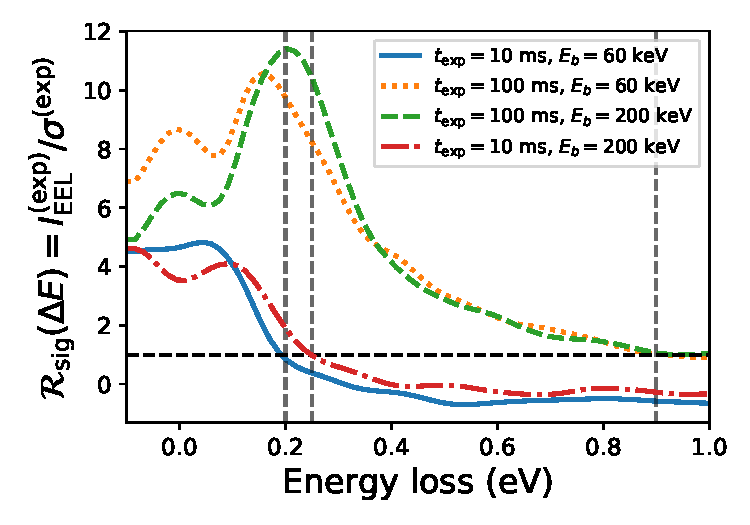
\includegraphics[width=120mm]{plots/intensity_to_error_ratio.pdf}
    \caption{The ratio between the central experimental value of the total
      EELS intensity, $I_{{\rm EEL},i}^{(\rm exp)}$, and the corresponding
      total uncertainty defined in Eq.~(\ref{eq:sigmaiexp}).
      %
      Results are shown for the four combinations of $t_{\rm exp}$
      and $E_{b}$ listed in Table~\ref{table:vacuumdata}.
      %
      The vertical dashed lines marks the values of $\Delta E$ for which
      this ratio becomes smaller than unity, which indicates when the input
      data starts to be dominated by the statistical noise.
      }
    \label{fig:intensityratio}
\end{figure}
%%%%%%%%%%%%%%%%%%%%%%%%%%%%%%%%%%%%%%%%%%%%%%%%%%%%%%%%%%%%%%%%%%%%%%%%%%%%%%%%%%%%%%%%%%%%%%%%%%%%%%%%%%%%%%%%%%%


Fig.~\ref{fig:intensityratio} displays this ratio
for the four combinations of $t_{\rm exp}$
and $E_{b}$ listed in Table~\ref{table:vacuumdata}.
%
The vertical dashed lines marks the values of $\Delta E$ for which
this ratio becomes smaller than unity.
%
For larger $\Delta E$, the EELS spectra become
consistent with zero within uncertainties and can thus be discarded and replaced
by the pseudo-data constraints.
%
The total uncertainty of the pseudo-data points is chosen to be
\be
\sigma_j^{(\rm pd)} = \frac{1}{10}I_{{\rm EEL}}^{\rm (exp)}\lp \Delta E = \Delta E_{\rm pd}^{\rm (min)}\rp \,, \quad 
j= 1,\ldots,N_{\rm pd} \, .
\ee
The factor of 1/10 is found to be suitable to ensure that the constraint
is enforced without distorting
the training to the experimental data.

The input data points listed in Table~\ref{table:vacuumdata} are used
to to generate a sample of $N_{\rm rep}=500$ Monte Carlo replicas
and train an individual neural network model to each of these replicas.
%
The end result of the procedure is a set of model replicas,
\be
\label{eq:modelreplicas}
I_{\rm ZLP}^{\rm (mod)(k)}(\Delta E, E_{b},t_{\rm exp}) \, , \quad k=1,\ldots,N_{\rm rep} \, ,
\ee
which can be used to provide a prediction for the intensity of the ZLP
for arbitrary values of $\Delta E$,  $E_{b}$, and $t_{\rm exp}$.
%
Eq~(\ref{eq:modelreplicas})
provides the sought-for representation of the probability density in the space of ZLP models.
%
For this sample of replicas one can evaluate
statistical estimators such as averages, variances, and correlations (as well
as higher moments) by means of
the usual expressions, for instance
\be
\label{eq:average}
\la I_{\rm ZLP}^{\rm (mod)}( \{z_1\}) \ra = \frac{1}{N_{\rm rep}}\sum_{k=1}^{N_{\rm rep}}
I_{\rm ZLP}^{\rm (mod)(k)}( \{z_1\}) \, ,
\ee
\be
\label{eq:standarddev}
\sigma_{I_{\rm ZLP}}^{\rm (mod)}( \{z_1\})  = \lp \frac{1}{N_{\rm rep}-1} \sum_{k=1}^{N_{\rm rep}}
\lp  I_{\rm ZLP}^{\rm (mod)(k)}  - \la I_{\rm ZLP}^{\rm (mod)}  \ra   \rp \rp^{1/2} \, ,
\ee
\be
\rho \lp \{z_1\},\{z_2\}\rp = \frac{ \la I_{\rm ZLP}^{\rm (mod)}( \{z_1\} ) I_{\rm ZLP}^{\rm (mod)}( \{z_2\} ) \ra
- \la I_{\rm ZLP}^{\rm (mod)}( \{z_1\} )\ra \la I_{\rm ZLP}^{\rm (mod)}( \{z_2\} ) \ra}{\sigma_{I_{\rm ZLP}}^{\rm (mod)}( \{z_1\} )\sigma_{I_{\rm ZLP}}^{\rm (mod)}( \{z_2\} )}
\ee
where as in the previous section $\{z_l\}$ denotes a possible set of input variables for the model.
We now discuss some of features of this ZLP vacuum model, here $\{z_l\}=\lp \Delta E, E_{b},t_{\rm exp}\rp$.

\subsection{Fit quality}
%
To begin with, we would like to quantify the overall fit quality of the model and demonstrate that it is flexible enough
to describe all the available input datasets.
%
In Table~\ref{table:chi2summary} we indicate the values of the final $\chi^2$ per data point,
    Eq.~(\ref{eq:chi2_final}), as well as the average values of the error Eq.~(\ref{eq:chi2})
    over the training and validation subsets, for each of the four sets of spectra listed in
    Table~\ref{table:vacuumdata} as well as for the total dataset.
    %
    We recall that for a satisfactory training one expects $\chi^2 \simeq 1$
    and $\la E_{\rm tr}\ra \simeq \la E_{\rm val}\ra \simeq 2 $~\cite{Forte:2002fg}.
    %
    From the results of this table we can see that these expectations are satisfied,
    both for the individual sets and for the total dataset.

    Then Fig.~\ref{fig:chi2_distributions} displays  the $\chi^2$  distributions
    evaluated for the training and validation sets
      of the $N_{\rm rep}=500$ replicas of the sample trained on the spectra
      listed in Table~\ref{table:vacuumdata}.
      %
      Note that the training/validation partition differs at random for each replica.
      %
      The $\chi^2_{\rm tr}$ distribution peaks at $\simeq 1$, indicating that a satisfactory model training
      has been achieved.
      %
      We emphasize that the stopping criterion for the neural net training adopted here never considers
      the numerical values of the error function and determines proper learning entirely from
      the global minima of $E_{\rm val}^{(k)}$.
      %
      From Fig.~\ref{fig:chi2_distributions}  we also observed that  $\chi^2_{\rm tr}$ distribution peaks at
      a slighter higher value, $\simeq 1.3$, and is broader that its corresponding training counterpart.
      %
      These results confirm both that a satisfactory model training that prevents overlearning
      has been achieved as well as an appropriate estimate of the statistical uncertainties
      affecting the original EEL spectra.
    
%%%%%%%%%%%%%%%%%%%%%%%%%%%%%%%%%%%%%%%%%%%%%%%%%%%%%%%%%%%%%%%%%%%%%%%%%%%%%%%%%%%%%%%%%%%%%%%%%%%%%%%%%%%%
\begin{figure}[t]
    \centering
    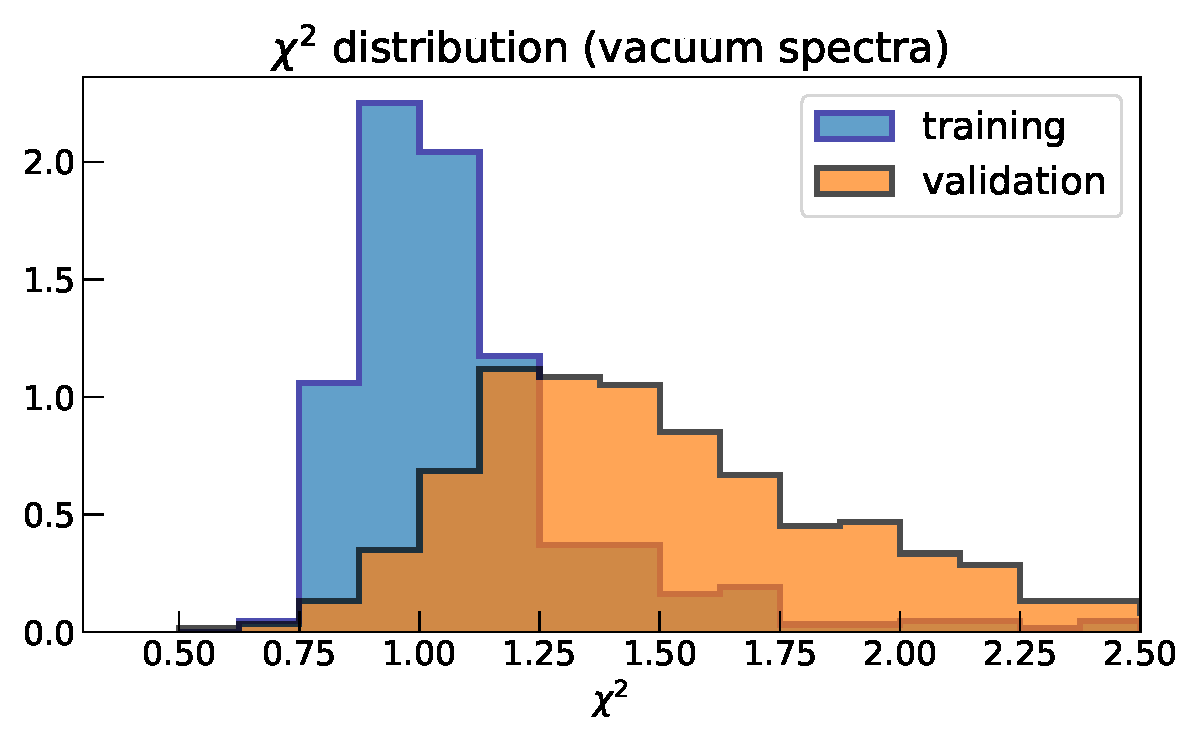
\includegraphics[width=120mm]{plots/chi2_distributions.pdf}
    \caption{The $\chi^2$ (per data point) distribution evaluated for the training and validation sets
      of the $N_{\rm rep}=500$ replicas of the sample trained on the spectra
      listed in Table~\ref{table:vacuumdata}.}
    \label{fig:chi2_distributions}
\end{figure}
%%%%%%%%%%%%%%%%%%%%%%%%%%%%%%%%%%%%%%%%%%%%%%%%%%%%%%%%%%%%%%%%%%%%%%%%%%%%%%%%%%%%%%%%%%%%%%%%%%%%%%%%%%%%%%%%%%%

%%%%%%%%%%%%%%%%%%%%%%%%%%%%%%%%%%%%%%%%%%%%%%%%%%%%%%%%%%%%%%%%%%%%%%%%%%%%%%%%%%%%%%%%%%%%%
%%%%%%%%%%%%%%%%%%%%%%%%%%%%%%%%%%%%%%%%%%%%%%%%%%%%%%%%%%%%%%%%%%%%%%%%%%%%%%%%%%%%%%%%%%%%%
\begin{table}[t]
  \begin{center}
            \renewcommand{\arraystretch}{1.35}
  \begin{tabular}{@{}cccc}
\br
Set & $\chi^2$  &  $\la E_{\rm tr}\ra$   &  $\la E_{\rm val}\ra$ \\
\mr
1        &                 &                  &    \\
2        &                  &                   &      \\
3        &                   &                   &     \\
4        &                   &                    &      \\
\mr
Total    &                     &                      &      \\
\br
  \end{tabular}
    \end{center}
  \caption{\small The values of the final $\chi^2$ per data point,
    Eq.~(\ref{eq:chi2_final}), as well as the average values of the error Eq.~(\ref{eq:chi2})
    over the training and validation subsets, for each of the four sets of spectra listed in
    Table~\ref{table:vacuumdata} as well as for the total dataset.
  }
   \label{table:chi2summary}
\end{table}
%%%%%%%%%%%%%%%%%%%%%%%%%%%%%%%%%%%%%%%%%%%%%%%%%%%%%%%%%%%%%%%%%%%%%%%%%%%%%%%%%%%%%%%%%%%%%%%%%5
%%%%%%%%%%%%%%%%%%%%%%%%%%%%%%%%%%%%%%%%%%%%%%%%%%%%%%%%%%%%%%%%%%%%%%%%%%%%%%%%%%%%%%%%%%%%%

\subsection{Dependence on the electron energy loss}
\label{eq:depdeltae}

Having demonstrated that our neural network model provides a satisfactory description
of all the input EEL spectra, we now present its  predictions for specific
choices of the input parameters.
%
First of all, we investigate the dependence of the results as a function of the
electron energy loss $\Delta E$.
%
In the left panel of Fig.~\ref{fig:EELS_vacuum_DeltaE} we show the central value and 68\% confidence level uncertainty band of the ZLP model as a function
of $\Delta E$,
evaluated using Eqns.~(\ref{eq:average}) and~(\ref{eq:standarddev}), for $t_{\rm exp}=100$ ms
and $E_{b}=60$ and 200 keV.
%
The inset displays the relative model uncertainty as a function of $\Delta E$.
%
We can observe the differences in the ZLP predictions as the electron beam energy $E_b$ is varied.
%
The relative uncertainties in the model turn out to be around 20\%, more or less independent
of the electron energy loss.

It is interesting to assess how the model results are modified once a subset of the data points
are excluded from the fit.
%
As illustrated in Fig.~\ref{fig:EELS_toy}, when training the model on sample spectra, a region
with $\Delta E_I \le \Delta E \le \Delta E_{II}$ will be removed from the training dataset to avoid the
contamination from the inelastic contributions.
%
To emulate the effects of such cut, in the right panel of Fig.~\ref{fig:EELS_vacuum_DeltaE} we
display the same comparison of the left one but now
for the case in which the input data bins with $\Delta E \ge 50$ meV are excluded from the fit.
%
In this way we test the extrapolation properties of the model between the data region ($\Delta E < 50$ meV)
and the region where $I_{\rm ZLP}(\Delta E)$ is forced to vanish.
%
If we compare the relative model uncertainties between the two cases, one can observe the expected
increase in the errors where a fraction of the input data has been cut away.
%
The same qualitative behaviour appears for the two values of $E_b$ considered here.
%
The comparisons of Fig.~\ref{fig:EELS_vacuum_DeltaE} indicate that our model uncertainties
indeed translate in an appropriate way the information contained in the training dataset -- note that
this would not be the case had one one a simple functional fit to model the ZLP.

%%%%%%%%%%%%%%%%%%%%%%%%%%%%%%%%%%%%%%%%%%%%%%%%%%%%%%%%%%%%%%%%%%%%%%%%%%%%%%%%%%%%%%%%%%%%%%%%%%%%%%%%%%%%
\begin{figure}[t]
    \centering
    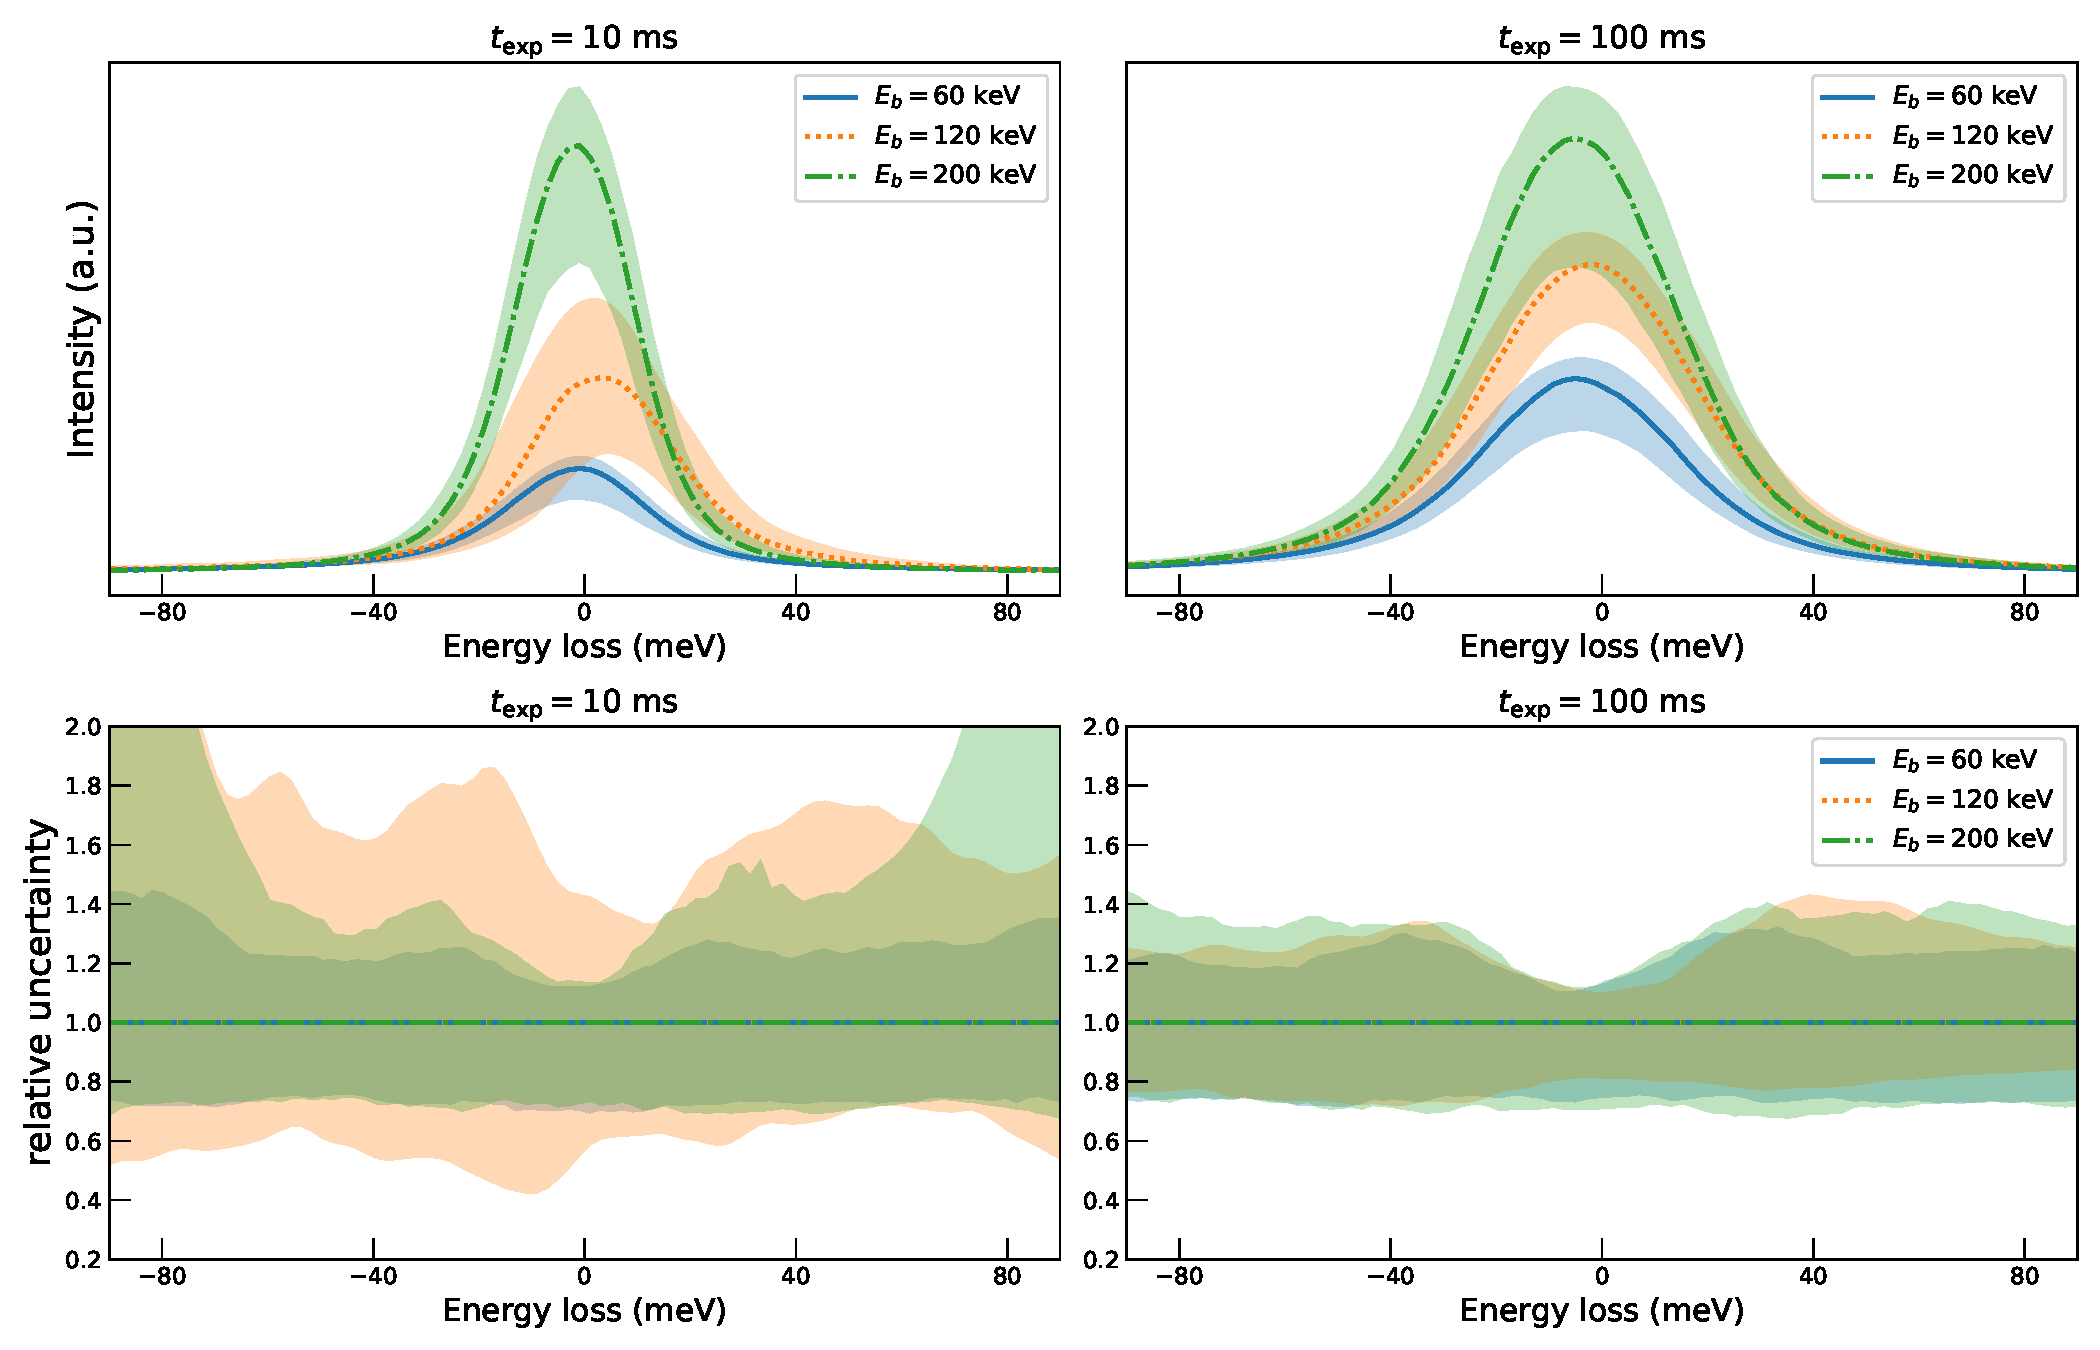
\includegraphics[width=170mm]{plots/deltaE_dependence_vacuum.pdf}
    \caption{Left panel: the central value and 68\% confidence level uncertainty band of the ZLP model as a function
      of electron energy loss $\Delta E$,
      evaluated using Eqns.~(\ref{eq:average}) and~(\ref{eq:standarddev}), for
      the three different values of $E_b$ considered and for both
      $t_{\rm exp}=10$ ms (left)  and $t_{\rm exp}=100$ ms (right panel).
      \label{fig:EELS_vacuum_DeltaE}}
\end{figure}
%%%%%%%%%%%%%%%%%%%%%%%%%%%%%%%%%%%%%%%%%%%%%%%%%%%%%%%%%%%%%%%%%%%%%%%%%%%%%%%%%%%%%%%%%%%%%%%%%%%%%%%%%%%%%%%%%%%

Fig.~\ref{fig:EELS_vacuum_DeltaE} displays
the relative uncertainty in the model predictions for $I_{\rm EEL}(\Delta E)$
as a function of the energy loss for $E_b=200$ keV and $t_{\rm exp}=10$ ms (left)
and 100 ms (right panel).
%
We show results for three different sets of trainings: without any cut
in the training dataset, and for the case where the data points with $\Delta E \ge \Delta E_{\rm cut}$
are removed from the training dataset for two different values
of $\Delta E_{\rm cut}$.
%
Note that the same pseudo-data points that enforce $I_{\rm EEL}(\Delta E)\to 0$ are present
in all three cases.

%%%%%%%%%%%%%%%%%%%%%%%%%%%%%%%%%%%%%%%%%%%%%%%%%%%%%%%%%%%%%%%%%%%%%%%%%%%%%%%%%%%%%%%%%%%%%%%%%%%%%%%%%%%%
\begin{figure}[t]
    \centering
    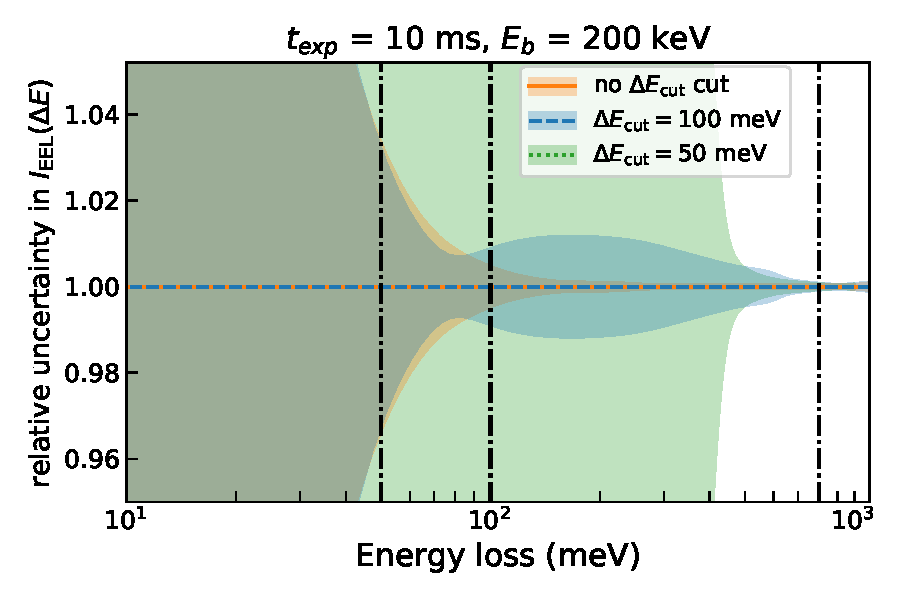
\includegraphics[width=0.49\textwidth]{plots/prediction_with_cut_10ms.pdf}
    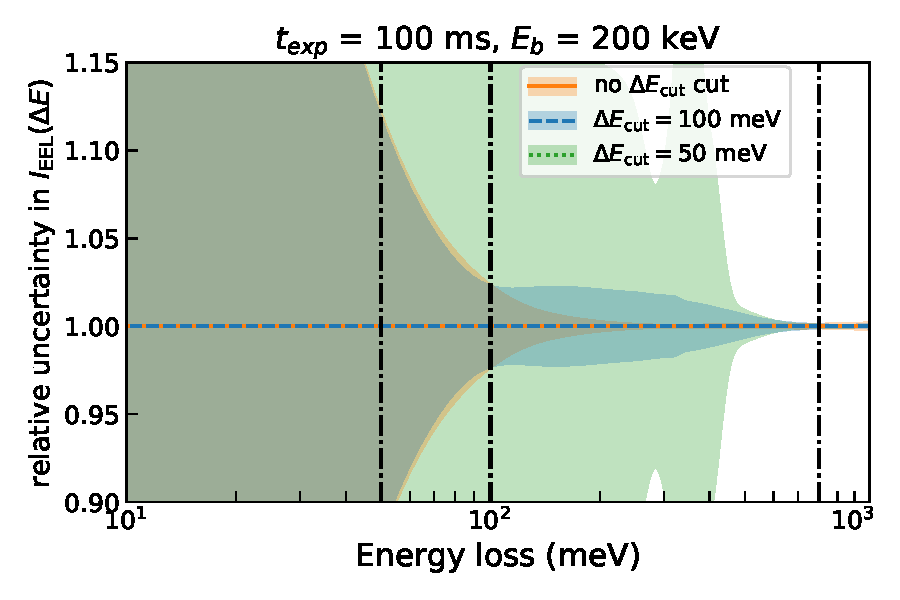
\includegraphics[width=0.49\textwidth]{plots/prediction_with_cut_100ms.pdf}
    \caption{The relative uncertainty in the model predictions for $I_{\rm EEL}(\Delta E)$
      as a function of the energy loss for $E_b=200$ keV and $t_{\rm exp}=10$ ms (left)
      and 100 ms (right panel).
      %
      We show results for three different sets of trainings: without any cut
      in the training dataset, and for the case where the data points with $\Delta E \ge \Delta E_{\rm cut}$
      are removed from the training dataset for two different values
      of $\Delta E_{\rm cut}$.
      %
      Note that the same pseudo-data points that enforce $I_{\rm EEL}(\Delta E)\to 0$ are present
      in all three cases.
      \label{fig:EELS_vacuum_DeltaE}}
\end{figure}
%%%%%%%%%%%%%%%%%%%%%%%%%%%%%%%%%%%%%%%%%%%%%%%%%%%%%%%%%%%%%%%%%%%%%%%%%%%%%%%%%%%%%%%%%%%%%%%%%%%%%%%%%%%%%%%%%%%

\subsection{Dependence on  beam energy  and exposure time }
\label{eq:depebeam}


As indicated in Table~\ref{table:vacuumdata}, the training dataset contains
spectra taken at two values of the electron beam energy, $E_b=60$ keV and 200 keV.
%
The left panel of Fig.~\ref{fig:extrapolbeam} displays  model predictions for the FWHM of the zero loss peak
      (and its corresponding uncertainty) as a function of the beam energy $E_b$
      for two values of the exposure time, $t_{\rm exp}=10$ ns and 100 ms.
      %
      The vertical dashed lines indicate the values of $E_b$ for which training data is available.
      %
      This comparison illustrates how the model uncertainty vary in the data region
      (near $E_b=60$ keV and 200 keV), the interpolation region (for $E_b$ between 60 and 200 keV),
      and the extrapolation regions (for $E_b$ below 60 keV and above 200 keV).
      %
      For $t_{\rm exp}=100$ ms, we observe that the model interpolates reasonably well
      between the measured values of $E_b$ and then uncertainties increase
      markedly in the extrapolation region above $E_b=200$ keV.
      
%%%%%%%%%%%%%%%%%%%%%%%%%%%%%%%%%%%%%%%%%%%%%%%%%%%%%%%%%%%%%%%%%%%%%%%%%%%%%%%%%%%%%%%
\begin{figure}[t]
    \centering
    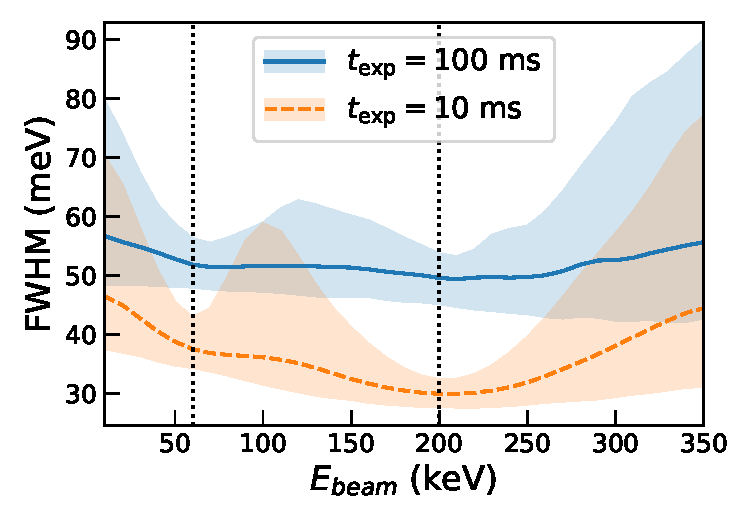
\includegraphics[width=0.49\textwidth]{plots/Ebeam_extrapolation.pdf}
    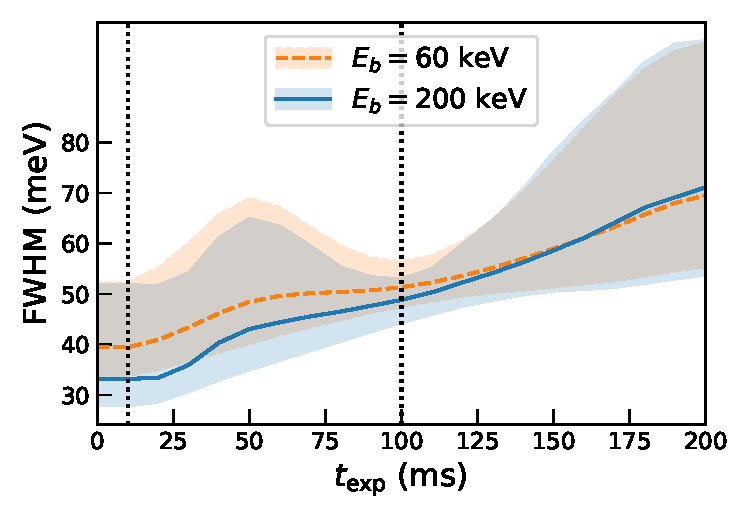
\includegraphics[width=0.49\textwidth]{plots/time_extrapolation.pdf}
    \caption{The model predictions for the FWHM of the zero loss peak
      (and its corresponding uncertainty) as a function of the beam energy $E_b$
      for two values of the exposure time (left panel)
      and as a function of $t_{\rm exp}$ for two values of $E_b$ (right panel).
      %
      The vertical dashed lines indicate the values of the
      corresponding parameter for which training data is available.
    }
    \label{fig:extrapolbeam}
\end{figure}
%%%%%%%%%%%%%%%%%%%%%%%%%%%%%%%%%%%%%%%%%%%%%%%%%%%%%%%%%%%%%%%%%%%%%%%%%%%%%%%%%%%%%%%%%%%%

For this comparison one can observe that as expected the uncertainty in the  prediction for FWHM
of the ZLP is the smallest close to the values of $E_b$ for which one has training data.
%
The uncertainties increase but only in a moderate way in in the interpolation region, indicating that
the model can be reliable applied to predict the features of the ZLP other values of the electron
energy beam (assuming that all other operation conditions of the microscope are unchanged).
%
The errors increase rapidly in the extrapolation region, which is a characteristic feature of
these neural network models.
%
Indeed, as soon as the model departs from the data region there exist a very large
number of different functional form models for $I_{\rm ZLP}(\Delta E)$ that can describe equally well
the training dataset, and hence a blow up of the extrapolation uncertainties is generically expected.

The network was trained on data with exposure times of $10$ and $100$ ms,
so interpolation and extrapolation is possible. Similar to the predictions for varying beam energy, also for exposure time the uncertainties grow bigger as the value deviates more from the training inputs.
%
The right panel of Fig.~\ref{fig:extrapolbeam} displays a similar model
comparison as in the left one but now and as a function of $t_{\rm exp}$ for two values of $E_b$ (right panel).
%
We observe that the FWHM increases roughly in a linear manner with the exposure time, indicating
that lower values of $t_{\rm exp}$ allow for an improved spectral resolution.
%
Further, also in this case we find that the model uncertainties grow rapidly in the
extrapolation region beyond that covered for the training dataset.


